%!TEX root = main.tex
\change{\section{Discussion of Study Results}}
To \change{further understand how participants
made use of the recommended visualizations during their analysis},
we analyzed the user study \change{transcripts}
through an open coding process~\cite{Muller1993} by two of the authors.
For each task in our study, we assigned a binary-valued code to indicate whether or not a participant engaged in a particular action or thought process. Table~\ref{table:thematic_summary} highlights results from thematic coding discussed in this section. We will use the notation [Participant.DatasetAlgorithm] to refer to a participant engaging with a dashboard created by an algorithm=\{1,2,3\}=\{\system, \cluster, \textsc{BFS}\} on a dataset =\{A,B\}=\{Police, Autism\}.
% \stitle{\system promotes distribution-awareness by provoking comparisons against more informative contextual references.}We first studied the thematic codes to understand how participants select contextual references for visualizations.
\subsection{The Choice of Contextual References}
\par As discussed earlier,
analysts often make use of
related visualizations to
form their \change{expectation or mental model} for
unseen \change{visualizations}.
We refer to \change{the}
visualizations used
for such purposes as \emph{contextual references}.
\change{The appropriate choice
of a contextual reference (such as an informative parent)
is necessary to ensure the \emph{safety} of
insights derived through drill-downs.}
To understand how ``safe'' the dashboards
generated from each condition were,
we examined \change{the visualizations}
that participants compared against
to \change{inform unseen visualizations}.
In particular, we thematically encoded
\change{the}
participants' use of contextual references
based on \change{their} verbal explanations
\change{for justifying} their prediction task responses.
As shown in Table \ref{table:contextualReferenceCount},
we find that participants make more comparisons in total using \system than \cluster and \BFS.
\begin{table}[h!]
\vspace{-5pt}
\centering
	\begin{tabular}{l|rrrr|r}
	 \small{Algorithm}   &    \small{Parent} &   \small{Sibling} &   \small{Relative} & \small{Overall} &   \small{Total} \\
	\hline
	 \small{\system}     &    \cellcolor{blue!25} 12 &       8 &     0 &  11 &      \cellcolor{blue!25} 31 \\
	 \small{\cluster}     &         4 &        0 &         7 &          8 &      19 \\
	 \small{\BFS}         &         0 &        5 &         1 &          8 &      14 \\
	\end{tabular}
\caption{Out of 12 participants, the number of participants who made use of each contextual reference across the two datasets. Participant behavior shows a similar trend in individual datasets. \system participants made more comparisons in general and against parents compared to the baselines.}
\label{table:contextualReferenceCount}
\vspace{-20pt}
\end{table}
\par Participants can (and often do) make comparisons against more than one type of contextual references to obtain their prediction. We uncovered four main classes of contextual references, described below using the
example visualization $V_i$=\texttt{\origcolor{gender=F,age=21-30}} (in the order of most to least similar to $V_i$): %and illustrated in Figure~\ref{fig:reference}:
\begin{enumerate}
	\item \textbf{Parent} : Comparison against a visualization with one
	filter removed (e.g., \texttt{\origcolor{gender=F}})
	\item \textbf{\achange{Sibling}} : Comparison against a visualization that shares the same parent. In other words, the \change{filtered attributes are the same, but one filter has a different value}. (e.g., \texttt{\origcolor{gender=F,age=}\diffcolor{60+}})
	\item \textbf{\achange{Relative}} : Comparison against a visualization that shares some common ancestor (excluding overall), but not necessarily the same parent. \change{These} visualizations share at least one \change{common filter, but with more than one filter or filter value being different}. (e.g., \texttt{\origcolor{gender=F,age=}\diffcolor{60+,race=White}})
	%\agp{I updated it based on what I thought this should have been--see figure for more}
	\item \textbf{Overall} : Comparison against the distribution that describes the overall population (no filters applied).
\end{enumerate}
% \begin{figure}[h!]
% \centering
% 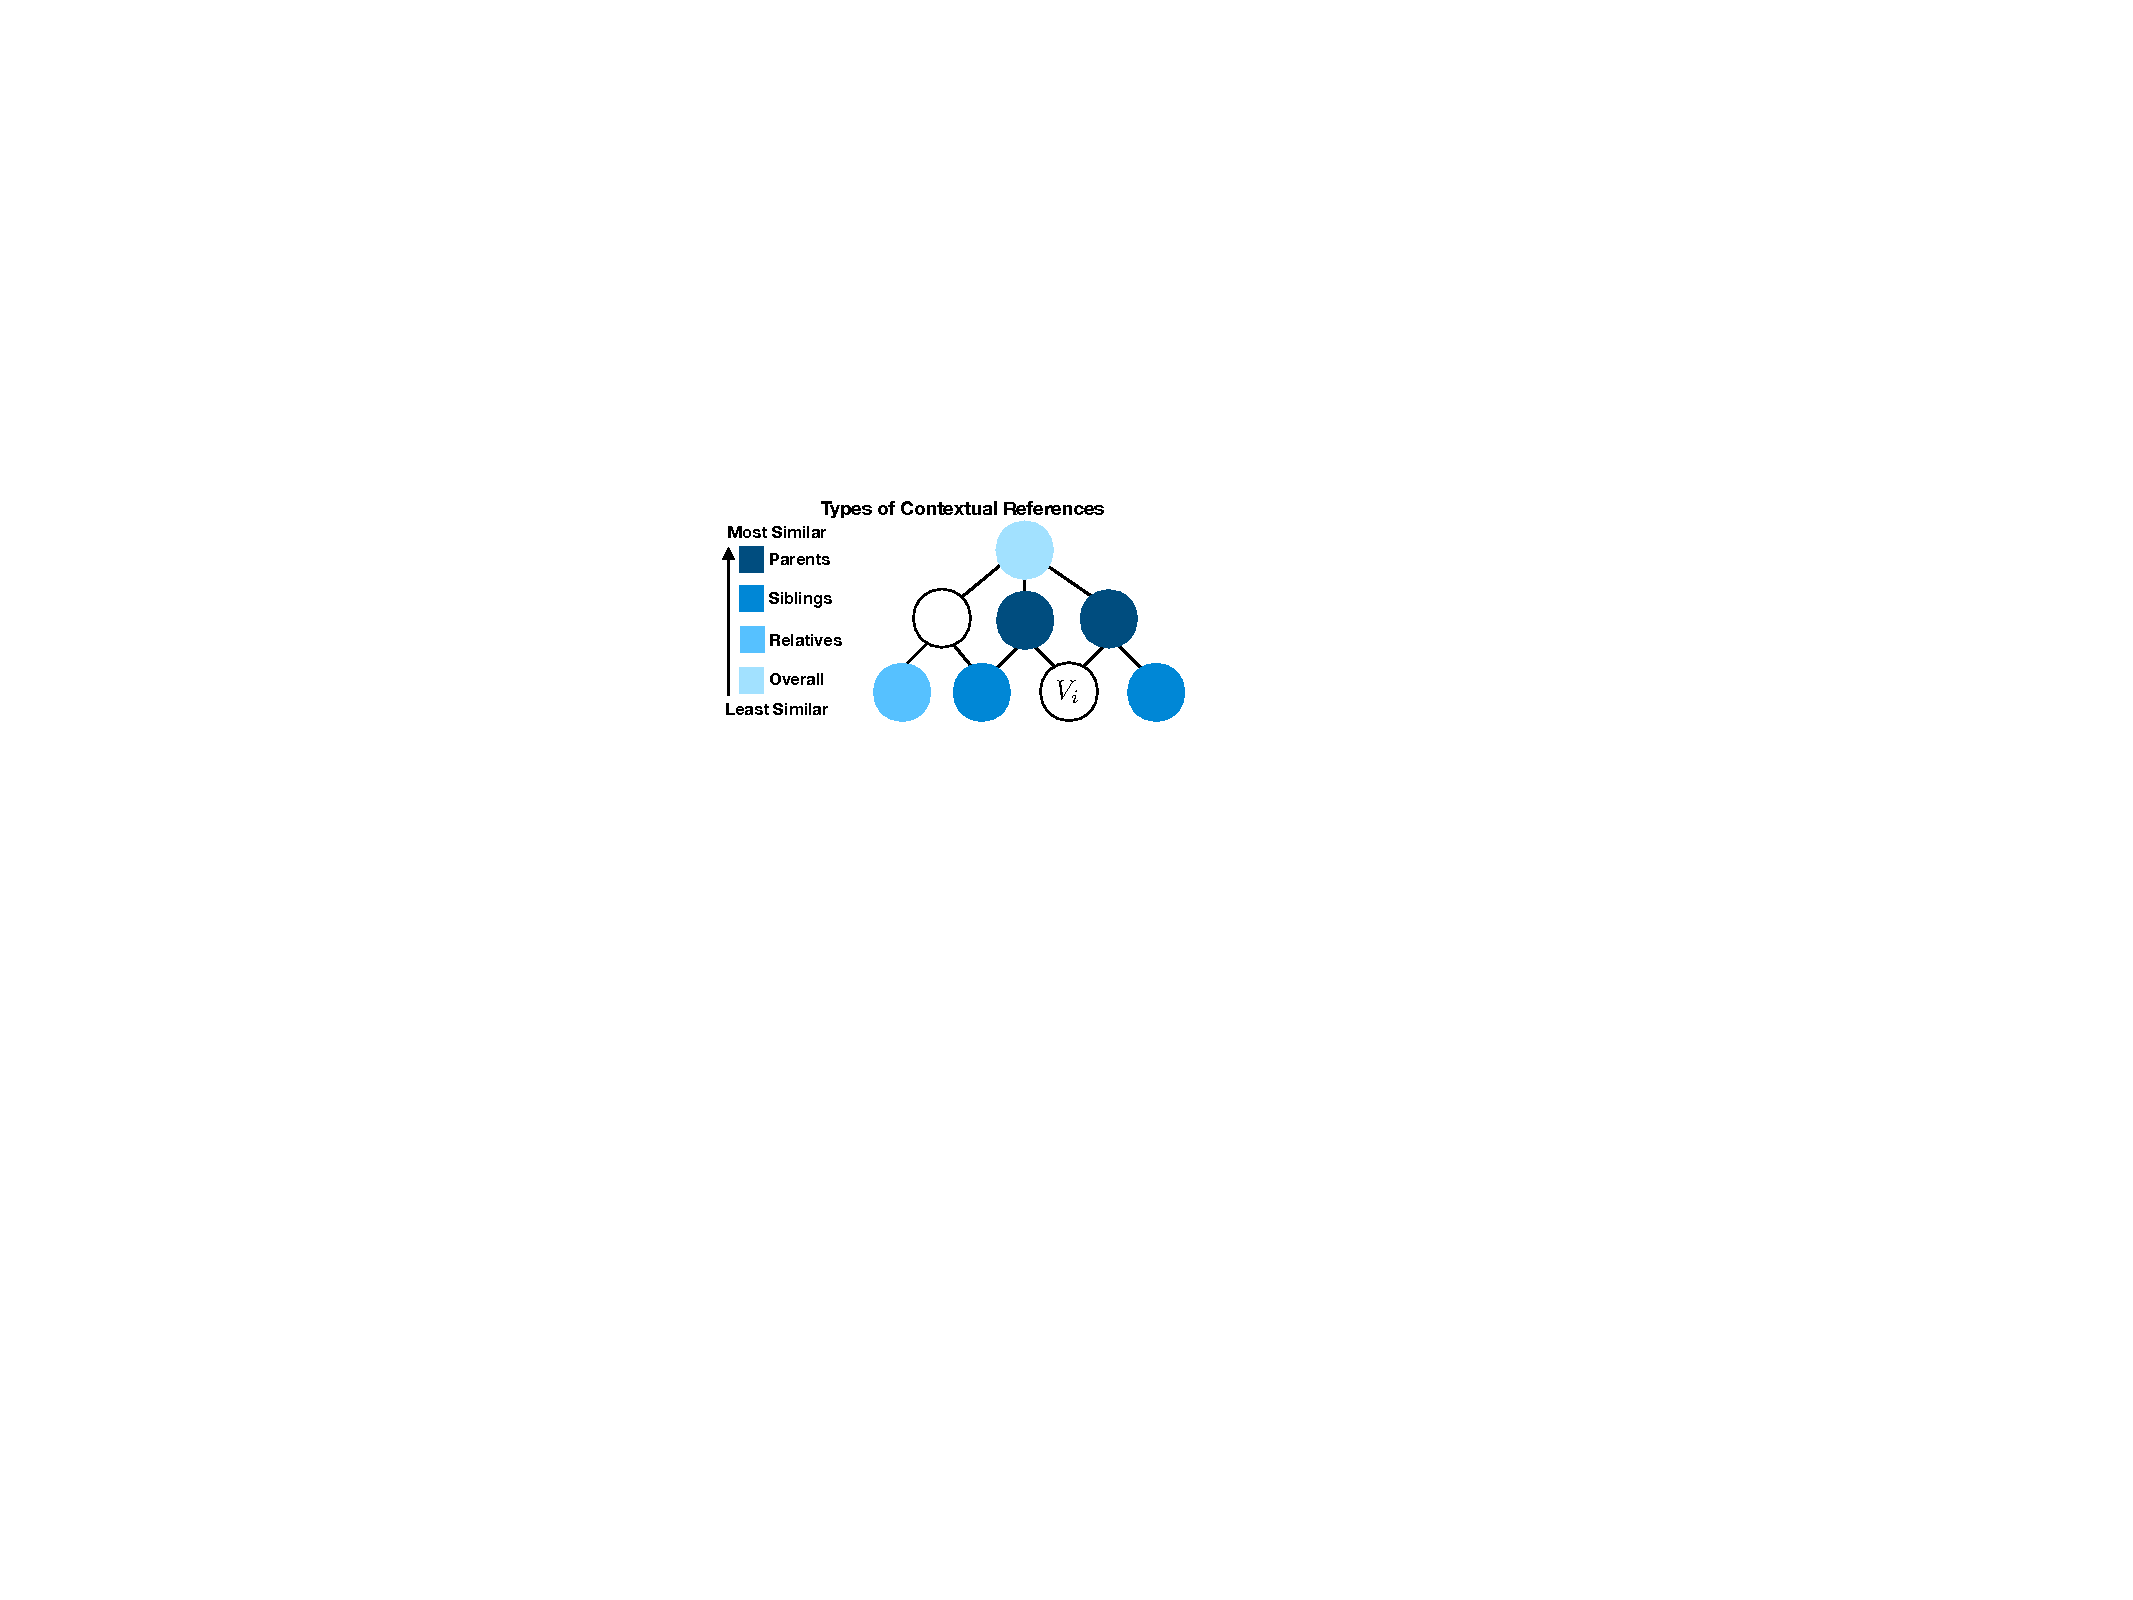
\includegraphics[width=0.7\linewidth]{figures/contextual_reference.pdf}
% \caption{\change{Different types of contextual references} for a given visualization of interest $V_i$. The degree of similarity with respect to $V_i$ is denoted by darkest to lightest color hue.\agp{I don't see how the relative is actually a relative. It shares no similarity with $V_i$, and is no different from the other white node. (One way to see this is that the common ancestor for both the so-called relative and the white node and $V_i$ are the same -- the overall one.)}}
% \label{fig:reference}
% \vspace{-10pt}
% \end{figure}
\par \change{Studying the participants' use of contextual references
reveals inherent challenges that arise from
using the \BFS and \cluster dashboards.}
For \cluster, participants mainly compared
against relatives and overall visualizations.
Since \cluster optimizes the diversity of distributions
amongst the \change{selected} visualizations,
\change{these} visualizations had up to 4 filters
and were disconnected from each other.
For this reason, in many cases\change{,}
participants could only rely on relatives
and the overall visualization as contextual references.
For example, P4.A2 pointed at a 4-filter visualization
with extreme values (100\% for warning; 0\% for arrest and ticket)
and indicated how ``\textit{a lot of} [the visualizations]
\textit{are far too specific. This is not very helpful.
You can't really hypothesize that all people are} \change{[sic]}
\textit{going to be warned, because it is such a specific category,
it might just be one person}''. %, you need to have a bigger dataset. And that category will not really give you such extremes to make it more credible''.
He further explained how he ``\textit{would not want to see the intersections} [visualizations with many filters] \textit{at first and would want to see all the bases} [univariate summaries] \textit{then dig in from there.}'' The lack of informative contextual references in the \cluster dashboard is also reflected in how analysts exhibited high variance and deviation in their prediction responses. %Note that the prediction task was chosen so that exactly one parent must be present in the dashboard, so these results do not point to the absence of parent visualizations in these \change{dashboards}, but rather indicate how participants made use of the information presented in the dashboards to form their prediction. \agp{I don't understand the previous sentence.}
\begin{table*}[ht!]
% \vspace{-10pt}
	%\centering\scriptsize
	\begin{tabular}{l|l|l|l}
	& \system & \cluster & \BFS \\ \hline
	Difficulty Interpreting Visualizations & 0 & \cellcolor[HTML]{FD6864}3 & 1 \\ \hline
	Misjudged Significance of Population Size & 0 & \cellcolor[HTML]{FD6864}4 & 1 \\ \hline
	Interpretable ``Human-like'' Dashboard & \cellcolor[HTML]{9AFF99}5 & 1 & 0 \\ \hline
	Number of Insights (Police) & \cellcolor[HTML]{9AFF99}11 & 8 & 9 \\ \hline
	Number of Insights (Autism) & \cellcolor[HTML]{9AFF99}16 & 6 & 11 \\
	\end{tabular}
\caption{Summary of qualitative insights from thematic coding. We record the total number of insights based on overall \change{dataset findings} that \change{were} independently discovered by more than two different participants. For each participant, we coded the absence or presence of 7 such insights for the Police dataset and 6 insights for the Autism dataset.}%findings regarding the dataset or information regarding one or more attributes
\label{table:thematic_summary}
\vspace{-20pt}
\end{table*}
\par Furthermore, \change{improper comparisons against contextual references often make} it difficult to \change{interpret} displayed visualizations. In particular, when visualizations composed of multiple filter conditions were shown in \cluster dashboards, 25\% of \change{the} participants had trouble \change{making sense of the meaning of a filter} for at least one of the datasets \change{(e.g., understanding that \texttt{gender=F AND age=60+} corresponds to female drivers with ages larger than 60 years old) at some point during the study}. In contrast, as shown in Table~\ref{table:thematic_summary}, this confusion only happened once for \BFS and none for \system. This is due to the fact that \cluster dashboards \change{seemed} random to the users, making it challenging to find ``close'' contextual references to compare against.
\change{In contrast, the linear ordering of \BFS and hierarchical ordering of \system were natural and interpretable for participants}. %In contrast, \BFS follows a linear ordering and \system follows a hierarchical ordering, which were more natural and interpretable for participants.
%despite our modification to KMeans which picks the visualizations with the least number of filters to show in the dashboard for improving interpretability
%These themes are drawn from user's explanations of how they obtained certain insights or ---- that --different tasks or while interpreting the dashboards. 4 categories :
\par For \BFS, most comparisons were based on the overall \change{visualization} and siblings. Due to the sequential level-wise picking approach, the overall visualization \achange{ corresponded to the immediate parent of all of the dashboard visualizations generated by \BFS (all of which are univariate distributions for $k=10$)}, so they are not explicitly recorded as a parent. While the overall and sibling comparisons can be informative, \change{the incomplete comparisons, due to the limited number of first-level visualizations displayed, can result in flawed reasoning, as observed
in the Autism prediction task.} In contrast, for \system, almost all users compared against the overall \change{one} and parents, while some also exploited \change{sibling comparisons} to make weaker guesses for less-frequently observed attributes (e.g., using a 2-filter sibling visualization involving \texttt{driver\_age} to infer another 2-filter visualization involving \texttt{driver\_age} with a different parent.)
% \subsection{Improper contextual reference can lead to misleading insights.}
% \subsection{The Danger of Improper References}%, echoing our previous concern regarding the danger of small subpopulation sizes. This issue stems from the fact that the contextual reference used for comparison was the overall population, however the unseen parent subpopulation may have behaved very differently.
\tr{
	\subsection{The Danger of Small Subpopulations}
	The danger of spurious patterns and correlations in visualizations that contain small subpopulation size is a well-known problem in exploratory analysis~\cite{Binnig2017}. When examining visualizations with many filters and extremely-skewed values in one or more bars (bars with 100\% or 0\%), 4 \cluster participants did not realize that charts with multiple filters may have a smaller subpopulation size. In contrast, 6 of the participants using \system explicitly noted that while these extreme-valued visualizations may be interesting, they were less certain due to the unknown subpopulation size and should be investigated further. For example, P1.A1 noted that a visualization with warning=100\% caught her eye, ``\textit{but I don't know what the N is, maybe it's one person, this makes me a little skeptical, that makes me want to go back to the raw data and look at what is the N and what drives something so drastic?}'' We also found that this subpopulation-size fallacy was observed to be more severe for the Autism dataset, where participants had less intuition on the expected attribute behavior.  Since \BFS dashboards only displayed first-level visualizations, participants for \BFS did not see visualizations with large numbers of filters that had small subpopulations during the study, so none of the \BFS participants exhibited signs of this fallacy.
}
% \subsection{Hierarchical layout leads to more natural contextual comparisons compared to table layout.}
%it was easier to follow contextual references in \system
\subsection{Interpretability of Hierarchical Layouts}
\par In the post-study interviews, participants cited hierarchical layout as \change{a} key reason \change{for why they preferred \system recommendations}. \change{Even though participants were never explicitly told what the edge connections between the visualizations meant during the study, they were able to interpret the meaning of the dashboards effortlessly through \system's hierarchical layout}. For example, P1.A1 stated that ``\textit{the hierarchical nature} [is] \textit{a very natural flow...so when you are comparing, you don't have to be making those comparisons in your head, visually that is very pleasing and easy to follow.}'' %Likewise, [P8.A1] also stated that ``I like the different levels, it makes it very visually easy to figure out what you want to look at, if you want to look at the overall data, it's right there at the top for you, if you want to get more specific, you just follow a branch downwards, which I think is very intuitive.''
Likewise, P9 described how \system's hierarchical layout for the Autism dataset was a lot easier to follow than the Police dataset shown in the table layout for \cluster:
\begin{quote}
\textit{If I had to look at this dataset in the format of the other one, this would be much more difficult. It was pretty hard for me to tell in the other one how to organize the tree, if there was even a tree to be organized. I like this layout much better, I think this layout allows me to approach it in a more meaningful way. I can decide, what do I think matters more: the overall trend? or the super detailed trends? and I know where to look to start, in the other one, every time I go back to it, I would say, where's the top level, where's the second level? I mentally did this. Like when you asked me that first question, it took much longer to find it, because I literally have to put every chart in a space in my head and that took a lot longer than knowing how to look at it.}
\end{quote}
At the end of the study, some participants \change{who were assigned dashboard conditions with \change{$5 \times 2$} table layouts \change{(i.e., \BFS and \cluster\ \achange{conditions})}} sketched and explained how they would like the layout of the visualizations to be done. \change{These} participants expressed that they wanted ``groupings'' or layouts that arranged visualizations with the same attribute together. Other participants advocated for isolating the overall visualization outside of the dashboard table for facilitating easier comparisons. Both of these suggestions provide further motivation for our hierarchical organization of visualizations. \change{\papertext{Our findings echo prior work on visualization sequences and storytelling~\cite{Hullman2017,Segel2010,Boy2015,Kim2017} in that analysts prefer visualization sequences structured hierarchically based on shared data properties, such as \achange{ordering by increasing levels of aggregation.}}}
%\agp{I don't understand what "ordered by increasing levels of summarization" is here, and why it makes sense}}}%, ordered by increasing levels of summarization.
%Kim et al.~\cite{Kim2017} modeled relationships between charts by empirically estimating transition (edge) cost between moving from one visualization (node) to another. They found that participants preferred ``\textit{starting from the entire data and introducing increasing levels of summarization}''.
 %layout and the idea of the collapsed visualizations as described earlier.%in Section \ref{sec:interaction}.
\par Since we did not inform participants about how the dashboards were generated, it was \change{surprising to see} that some participants \change{presumed} that \achange{certain} dashboards were hand-picked by a human analyst and \change{hypothesized} what this \change{fictitious analyst}'s intentions were (e.g., ``\textit{It seems like the researcher who created this dashboard was specifically looking at people of Asian descent and people who are 60 or older.}'' [P7.A1]). \change{Table~\ref{table:thematic_summary} shows how} 5 out of 12 participants referred to the \system dashboards as if they were generated by a human, whereas only 1 participant for \cluster and none for \BFS made such remarks\change{\footnote{We encoded this phenomenon by looking at instances where a participant either explicitly \change{referred} to a person who picked out the dashboard or implicitly described their intentions through personal pronouns.}}. At the end of the study, many were surprised to learn that the \system dashboard was actually picked out by an algorithm, indicating that \system could automatically \change{generate convincing dashboards similar to ones that were} authored with human intention. The interpretability of \system dashboards may have contributed to the increased number of insights discovered in both datasets compared to the two baselines, as summarized in Table~\ref{table:thematic_summary}.
\subsection{Limitations of \system}
% Interestingness task is highly subjective, so not conclusive whether interesting or not , despite the positive result
% Due to the highly subjective nature of the retrieval task, the interestingness selection for the Police dataset was biased by participant's priors and intuition about the attributes. For example, while all participants who have seen the visualization "duration=30+min" verbally noted that stop duration is a crucial factor that leads to arrest, only 4 users marked it as interesting. 5 participants marked the visualization as not interesting and 4 left it unselected, because the visualization was not very surprising as it agreed with their intuition that ``\textit{if the police stop is taking a long time, something has probably gone wrong}''.
\par As described earlier, since the details of how the dashboards were obtained \change{were} not explained to the users during the study, some users expressed that they were initially confused by \system\ \change{as} not all variables were present in the dashboard. Others also found it confusing that the addition of filters did not always correspond to the same variables. For example, P2.A1 \change{felt that} the dashboard was intentionally biased:
\begin{quote}
\textit{I feel like this one, not all the data is here, so we are already telling a story, you are trying to steer the viewer to look at certain things. And the focus seems to be on where the arrest rate is high. You probably could have found other things that led to ticket being high, but you didn't pull those out. You are trying to see if there are other factors that lead to more arrests.}
\end{quote}
\npar This sentiment is related to participants' desire to perform their own ad-hoc querying alongside the dashboard to inspect other related visualizations for verifying their hypothesis. For example, P7.A1 wanted to inspect all other first-level visualizations for driver's race to assess its influence. P7.A1 expressed that while he had learned many insights from the dashboard, ``\textit{the only thing I don't like is I cannot control the types of filter, which is fixed.}''
\change{Since our current goal was to simply provide an informative dashboard and evaluate its utility,
the present version of \system is limited in its interactivity and the extent of free-form data exploration it supports. This result also points to how} \system could serve as a helpful \change{assistant} alongside other conventional visualization tools, such as Tableau. Outside the context of the user study, it is essential to explain how \system\ \change{selects} the visualizations in \change{an} easy and interpretable manner to establish a sense of \bchange{the
summarization objectives} for the users and
help them make better inferences with the dashboard.

\change{%a small set of analytic tasks corresponding to each design objectives, with
Since the goal of our study is to evaluate whether \system can assist users in drill-down exploration, our preliminary study is limited to comparisons against baselines stemming from conventional approaches for multidimensional data exploration. While we understand how the \system study condition may confound the hierarchical layout with the algorithmic choice of visualizations, our intention for the baseline
was to simulate how analysts generate a large number of visualizations individually, typically arranged in a table grid layout, rather than using a hierarchical layout. Further evaluation comparing how different hierarchically-displayed visualization selection algorithms assist users in drill-down exploration is a direction of future work.
}
\tr{
	\par As discussed earlier, subpopulation size is important in establishing the significance of a trend observed in a visualization. While subpopulation size is taken into account implicitly in our objective, we should design interfaces that convey the notion of subpopulation size in our dashboard. Examples include Sankey-like flow diagrams indicating the percentage of the parent population broken down into individual subpopulations and subpopulation size explicitly specified via edge labels.
}


%, either explicitly displayed as text when hovering over the visualization or changing the size or background color of the visualizations to encode subpopulation size.
%“I actually found it really confused at first because such a low arrest rate at the top, and then at the bottom the arrest rate was much higher, so I was like is this data wrong. Then I realized we’re not looking at all the data here, you’ve pulled out some of it. It took me a minute to realize that. And once I read the title of the charts I realized that makes sense.” [P2.A1]
% - Reference of Comparison
% - Layout naturally lends itself for comparison:
% 	- describe ordering layout, how participants naturally follow the flow
% 	- emph that we did not tell them what the edge connections mean and how they were computed but the users naturally figured it out, that it means adding an additional filter.
% 	- hierarchical interpretable nature (quotes)
% 	- compared to other baselines
% 	- describe dashboard by human (count)
% - Misleading insights v.s. True insight discovery rates
% 	- Interpretability:
% 	- misled understanding subpopulation size
% 		- for autism, it is important to see if they compare to overall because if not they would think high skew to NO is important whereas its actually pretty close to overall.
% 	- trouble interpreting filter combination
%%%%%%%%%%%%%%%%%%%%%%%%%%%%%%%%%%%%%%%%%%%%%%%%%%%%%%%%%%%%%%%%%%%%%%%%%%%%%%%%%%%%%%%%%%%%%%%%%%%%%%%%%%%%%%%%%%%%%%%%
%%%%%%%%%%%%%%%%%%%%%%%%%%%%%%%%%%%%%%%%%%%%%%%%%%%%%%%%%%%%%%%%%%%%%%%%%%%%%%%%%%%%%%%%%%%%%%%%%%%%%%%%%%%%%%%%%%%%%%%%
%%%%%%%%%%%%%%%%%%%%%%%%%%%%%%%%%%%%%%%%%%%%%%%%%%%%%%%%%%%%%%%%%%%%%%%%%%%%%%%%%%%%%%%%%%%%%%%%%%%%%%%%%%%%%%%%%%%%%%%%
% \subsection{Statistical Paradoxes}\dor{make title full sentences}
% Visualizations are powerful representations for studying different distributions or patterns in a dataset, but our human intuition could often mislead us when it comes to interpreting those patterns\cite{Binnig2017,Wall2017}. Several statistical paradoxes can lead analysts to draw incorrect conclusions from observed visualizations, including Simpson's paradox as discussed in the introduction. The key reason why many of these paradoxes emerge is the \emph{incompleteness} of the observed data or lack of focus on relevant informative subsets of the data. For example, Simpson's paradox arises in the presence of an unseen confounding variable. %likewise, the absence of  base rate information causes base rate fallacy.
%  We assert \dor{too strong of a sentence} that distributional awareness can be useful in avoiding such statistical paradoxes. If an analyst is aware of all distributions in a given dataset, he/she is less prone to many statistical paradoxes. However, given the large number of dimensions and high cardinality of these dimension in modern datasets, it is not possible for an analyst to explore and memorize all distributions. Therefore, a more evolved approach is to be aware of the exceptional distributions. In this work, we propose a first step towards this goal, where we identify the exceptional distributions in terms of their informative references. The remaining (unseen) distributions in the dataset are rather unsurprising and can be inferred from the visualizations in the dashboard. \dor{I would recommend first talk about issue with large dimension + danger of multiple hypothesis testing + incomplete testing, point out problem, then talk about how our system resolves this.}
% \subsection{Structural Insight}
% Our proposed dashboard consists of a hierarchy of visualizations, where each visualization is linked to its most informative parent. The shape or structure of the hierarchy contains useful information that augments the information learned from the visualizations and aid distribution awareness and understanding. \dor{what's interesting here is that while many work have looked at visualization presentation, layout of presentation never considered, we find in Sec 5 that this is actually important and can encode info.} For example, the depth and branching factor of the hierarchy could inform a user regarding the configuration of insights. Deep hierarchies contain long paths, i.e., insights are present at lower level visualizations with multiple constraints. In contrast, bushy hierarchies (with high branching factor) contain cases where multiple visualizations have the same informative parent and they differ from that parent. \dor{do we have examples from the study that support this?} We assert that the depth and branching factor could be a meaningful constraint in our problem formulation \dor{too strong of a sentence}. Some applications for example, funnel exploration require studying deep hierarchies, whereas others for example, building decision trees require studying bushy hierarchies. A natural extension of our current problem formulation is to allow users to select the depth and branching factor for the hierarchy.
% \subsection{Other Visualization Lattices}
% In this work, we explore the space of data subsets to generate our visualization lattice. Note that it is possible to explore the space of dimension attributes in x-axis to generate a different visualization lattice. In particular, given a combination of dimension attributes $X = \{X_1, \ldots, X_n\}$, adding one or more new dimensions in $X$ will generate a new combination. An ancestor-descendant relationship exists between these dimension combinations, following the same principles of Section 3.1. These relationships lead to a new lattice, which we call the dimension combination lattice. Our informative deviation based approach could be used for traversing the dimension combination lattice. However, we observe that most users do not visualize more than two attributes in x-axis. Therefore, traversing the dimension combination lattice is not very useful for most applications.
% \dor{I think 6.2,6.3 don't tie well with the rest of the paper. It sounds like stretching our own ideas rather than being motivated by the work done in this paper. Other potentially more relevant discussion: distribution awareness and how it might be useful in other contexts? Decision trees?}
% %\subsection{Utility Metrics}
